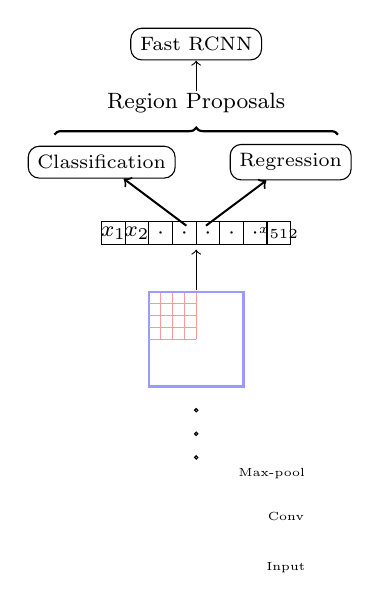
\begin{tikzpicture} [scale=0.30,rotate=90]  
	% \onslide<1>{\draw[draw=red!50,fill=red!10,thick,solid,rounded corners] (-2,-6) rectangle (11.5,3); }
	% \onslide<2>{\draw[draw=red!50,fill=red!10,thick,solid,rounded corners] (15,-8.5) rectangle (19.5,6); }
	%\onslide<3>{\draw[draw=red!50,fill=red!10,thick,solid,rounded corners] (20,-5) rectangle (24,3); }
	
	\onslide<1->{

		\renewcommand{\forefillColor}{black!50!white}
		\renewcommand{\borderColor}{white}
		\renewcommand{\toprsidefillcolor}{red}

		%% input layer
		\handmadecube{0}{4.5}{2.5}{-1}{0}
		\renewcommand{\toprsidefillcolor}{green}                  
		\handmadecube{0}{4.5}{2.5}{-1+0.2}{0}
		\renewcommand{\toprsidefillcolor}{blue!60!white}          
		\handmadecube{0}{4.5}{2.5}{-1+0.4}{0}
		\node[scale=0.85] at (1-0.6*2.6-0.1,0-4.8){\tiny{Input}};
		%     \node [scale=0.7, rotate=45] at (1-0.6*2.6+0.6,0.2) {\tiny{224}};
		%     \node [scale=0.7, rotate=90] at (1-0.6*2.6+0.2,-2) {\tiny{224}};


		% Convolution Layer
		\renewcommand{\forefillColor}{red!50!white}
		\renewcommand{\borderColor}{white}
		\renewcommand{\toprsidefillcolor}{red!50!white!50}

		\pgfmathsetmacro{\seedx}{1}
		\pgfmathsetmacro{\seedy}{0}

		\foreach \xct/\yct in {1,...,2}
		{
			\pgfmathsetmacro{\xcti}{\seedx+\xct*0.1}
			\pgfmathsetmacro{\ycti}{\seedy}
			\handmadecube{0.5}{4.5}{2.5}{\xcti}{\ycti}
		}
		\node[scale=0.85] at (1+0.5,0-4.8){\tiny{Conv}};
		%     \node [scale=0.7, rotate=45] at (1-0.6*2.6+3.2,0.2) {\tiny{224}};
		%     \node [scale=0.7, rotate=90] at (1-0.6*2.6+0.2+2.6,-2) {\tiny{224}};
		
		%     \node[scale=0.7] at (1+0.725,0-4.2){\tiny{64}};
		
		
		
		% Pooling Layer
		\renewcommand{\forefillColor}{blue!50!white}
		\renewcommand{\borderColor}{white}
		\renewcommand{\toprsidefillcolor}{blue!50!white!50}
		
		\pgfmathsetmacro{\seedx}{2.5}
		\pgfmathsetmacro{\seedy}{0}

		\foreach \xct/\yct in {1}
		{
			%       \pgfmathsetmacro{\xcti}{\seedx+\xct*0.1}
			%       \pgfmathsetmacro{\ycti}{\seedy}
			
			\pgfmathsetmacro{\xcti}{\seedx+\xct*0.1}
			\pgfmathsetmacro{\ycti}{\seedy}
			\handmadecube{0.5}{3.8}{1.8}{\xcti}{\ycti}
		}
		\node[scale=0.85] at (0.5+2.8,0-4.2){\tiny{Max-pool}};
		%     \node [scale=0.6, rotate=45] at (1+3.7,0.2) {\tiny{112}};
		%     \node [scale=0.6, rotate=90] at (1+3.3,-2+0.5) {\tiny{112}};
		%     \node[scale=0.7] at (1+2.85,0-3.5){\tiny{64}};
		
		\foreach \xct in {1,2,3}
		{
			\filldraw[fill=gray!60](3+\xct,-1) circle(2pt) ;
		}

		\draw [thick,step=1,draw=blue!40!white](7,-3) rectangle (11,1);
		\draw [thin,step=0.5,draw=red!40!white](9,-1) grid (11,1);
		\draw [thin,step=0.5,draw=red!40!white](9,-1) -- (9,1);

		%     \filldraw[fill=green!50!white, draw=black,rounded corners] (13,4) rectangle (14,5);
		\draw [thin,step=1,draw=blue!40!white](7,-3) rectangle (11,1);
		\draw (13,-5) grid[xstep=1,ystep=1] (14,3);     
		\node (x1) at (13.5,2.5) {\footnotesize{$x_1$}};
		\node (x2) at (13.5,1.5) {\footnotesize{$x_2$}};

		\foreach \y in {1,2,...,5}{
			\node (x2) at (13.5,1.5-\y) {\footnotesize{$\cdot$}};
		}

		\node (x2) at (13.5,-4.5) {\tiny{$x_{512}$}};

		\draw[->](11.1,-1)--(12.8,-1);

		\node(A) at (13.5,-1){};
		\node(B)[draw,rounded corners] at (16.5,3){\scriptsize{Classification}};
		\node(C)[draw,rounded corners] at (16.5,-5){\scriptsize{Regression}};
		\node(D)[draw,rounded corners] at (21.5,-1){\scriptsize{Fast RCNN}};
		\path[draw,line width=0.25mm,->] (A) edge (B);
		\path[draw,line width=0.25mm,->] (A) edge (C);
		%\node(D)[draw,rounded corners] at (20.5.5,3){\scriptsize{Classification}};
		\draw[->](19.5,-1)--(20.8,-1);
		\node[font=\fontsize{8}{10}\selectfont] at (19,-1) {Region Proposals};

           
		\draw [
			thick,
			decoration={
				brace,
				raise=0.2cm
			},
			decorate
		] (17,5) -- (17,-7) 
		node [pos=0.1,anchor=north,xshift=-0.5cm,yshift=1.1cm] {};
		

	}
\end{tikzpicture}
